
\section{Modellierung}
    Um Differentialgleichungen eines Systems herzuleiten:
    \subsection{Arten der Modellierung}
        \subsubsection{Impulserhaltung}
            \[\frac{d}{dt}(m\dot{x}) = \Sigma_i F_i\]
        \subsubsection{Drehimpulserhaltung}
             \[\frac{d}{dt}(J_B\dot{\theta})= \Sigma_i T_i\]
        \subsubsection{Speichermethode}
          \[\frac{d}{dt}(\textrm{Speicherinhalt}) = \sum \textrm{Zuflüsse} - \sum \textrm{Abflüsse}\]
		\subsubsection{Vorgehen}
		    \begin{enumerate}
    		       
    		    \item  Identifiziere die Systemgrenze (Zuflüsse, Abflüsse)
    
    		    \item  Identifizieren die relevanten Speicher im System (Masse, Energie, Ladung) 
    
    		    \item  Formuliere die DGL
    
     			    $\frac{d}{dt}(\textrm{Speicherinhalt}) = \sum \textrm{Zuflüsse} - \sum \textrm{Abflüsse}$
    
    	    	\item  Formuliere algebraische Relationen der Zuflüsse/Abflüsse eines Speichers als Funktion der Pegelvariablen. %Nach einsetzten sollten sowohl der Speicherinhalt wie auch 				die Zuflüsse/Ausflüsse als Funktion der Pegelvariablen ausgedrückt sein. 
    
    	    	\item  Identifizieren Systemparameter durch Experimente, Designspezifikationen oder Systemoptimiereung
    
    	    	\item  Validiere das Modell mit Experiment
		    \end{enumerate}

    \subsection{Zustandsgleichung}
	    von nicht-linearer DGL in eine Zustandsgleichung erster Ordnung. 
 	    \[\vec{z} = \begin{bmatrix} z \\ z' \\ z'' \\ \vdots \\z^{n-1} \end{bmatrix}  = \begin{bmatrix} z_1 \\ z_2 \\ z_3 \\ \vdots \\z_n \end{bmatrix}
         \xrightarrow{\frac{d}{dt}} \vec{\dot{z}} = \begin{bmatrix} z' \\ z'' \\ z''' \\ \vdots \\z^{n} \end{bmatrix} = \begin{bmatrix} f_1 \\ f_2 \\ f_3 \\ \vdots \\q(z_n,\hdots,z_2,z_1,v) \end{bmatrix}\]
         
    \subsection{Normierung}
        Die Grössen im Zustandsvektor $\vec{z}$ weisen verschiedene Einheiten auf. Durch Normierung erhalten wir eine vereinfachte Interpretation und beugen numerische Probleme vor. 
        \[z_i(t) = z_{i,0}\cdot x_i(t), \quad z_{i,0} \in\mathbb{R}\setminus\{0\} \] 
        \textbf{in Vektornotation:}
        \[ z = T \cdot x, \hspace{5mm}  T = \textrm{diag}(z_{1,0},\hdots,z_{n,0})\] 
        \[\Rightarrow x=T^{-1}z\]
    
        Die Ein- und Ausgangsgrössen werden analog normiert:
        \[v(t) = v_0 \cdot u(t) \hspace{5mm} v_0 \in\mathbb{R}\setminus\{0\}\]
        \[w(t) = w_0 \cdot y(t) \hspace{5mm} w_0 \in\mathbb{R}\setminus\{0\}\]
    
        Generell gilt
        \[T \cdot \dot{x} = \dot{z} = f(z,v) \]
        \[w_0 \cdot y = w = g(z,v)\]

\vfill\null\columnbreak
        Nun normiert man das System:
    
        \[ \dot{x} = T^{-1} \cdot f(T \cdot x, v_0 \cdot u) = f_0(x,u) \]
        \[ y = w_0^{-1} \cdot g(T \cdot x, v_0 \cdot u) = g_0(x,u)\]
   
        Die normierte Gleichung $\dot{x} = T^{-1} \cdot f(T \cdot x, v_0 \cdot u) = f_0(x,u)$ hat Einheit: $[\frac{1}{s}]$.
    
    \subsection{Linearisierung}
    
    Nach Normierung wird das System um den Gleichgewichtspunkt linearisiert. 
    
    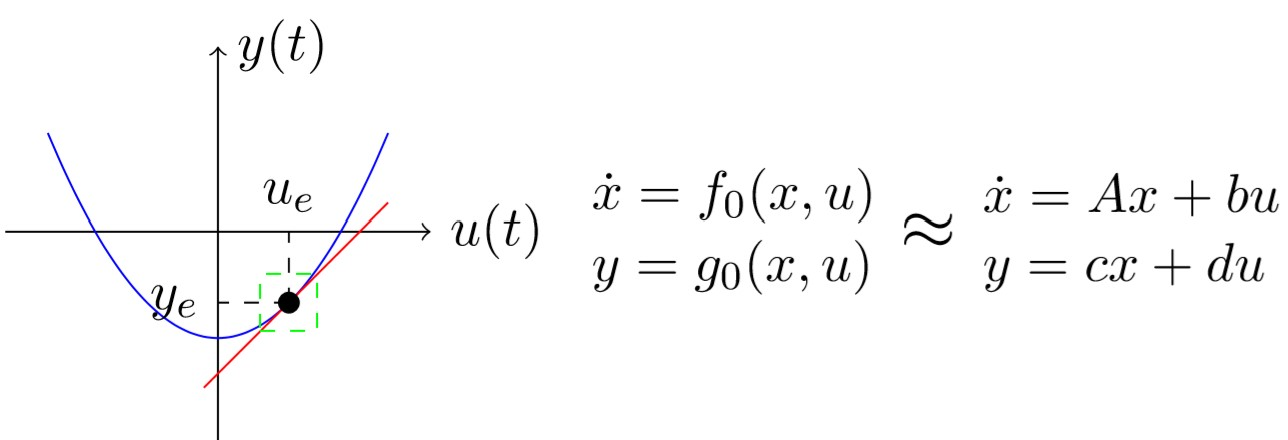
\includegraphics[width=\linewidth, height=30mm]{images/01/01_linearisierung.jpg}
    Um das System zu linearisieren wird zuerst die Gleichgewichtslage berechnet. Im Gleichgewichtszustand gilt per Definition:
    \[ \dot{x} = \begin{bmatrix} \dot{x}_1 \\ \vdots \\ \dot{x}_n\end{bmatrix} = \begin{bmatrix} 0 \\ \vdots \\ 0 \end{bmatrix} = f(x_e,u_e)\]
    
    Dies ist ein lineares Gleichungssystem in $x_1,x_2,...,x_n$ und $u$. Für einen gewünschten Zustand $x_e$ lässt sich ein $u_e$ berechnen. Dabei ist zu beachten, dass nicht alle gewünschten $x_e$ möglich sind. Umgekehrt lässt sich für ein konstantes $u_e$ der resultierende Gleichgewichtszustand $x_e$ berechnen.
    
    Um das System um den Gleichgewichtspunkt zu linearisieren, werden die Matrizen A,b,c,d berechnet:
    
    \begin{center}
        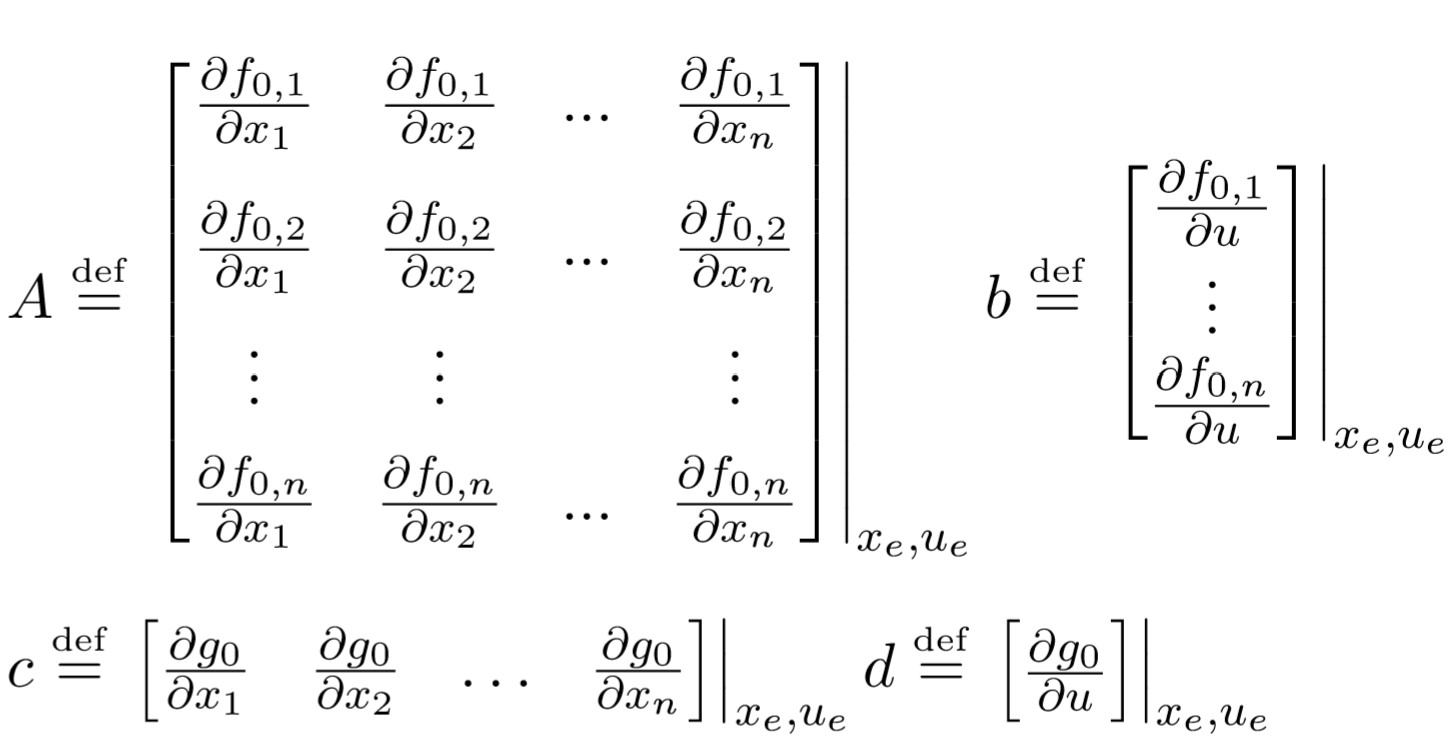
\includegraphics[width=\linewidth]{images/01/01_Statespace.jpg}
    \end{center}
    
    \subsection{Entlinearisierung}
        \begin{center}
            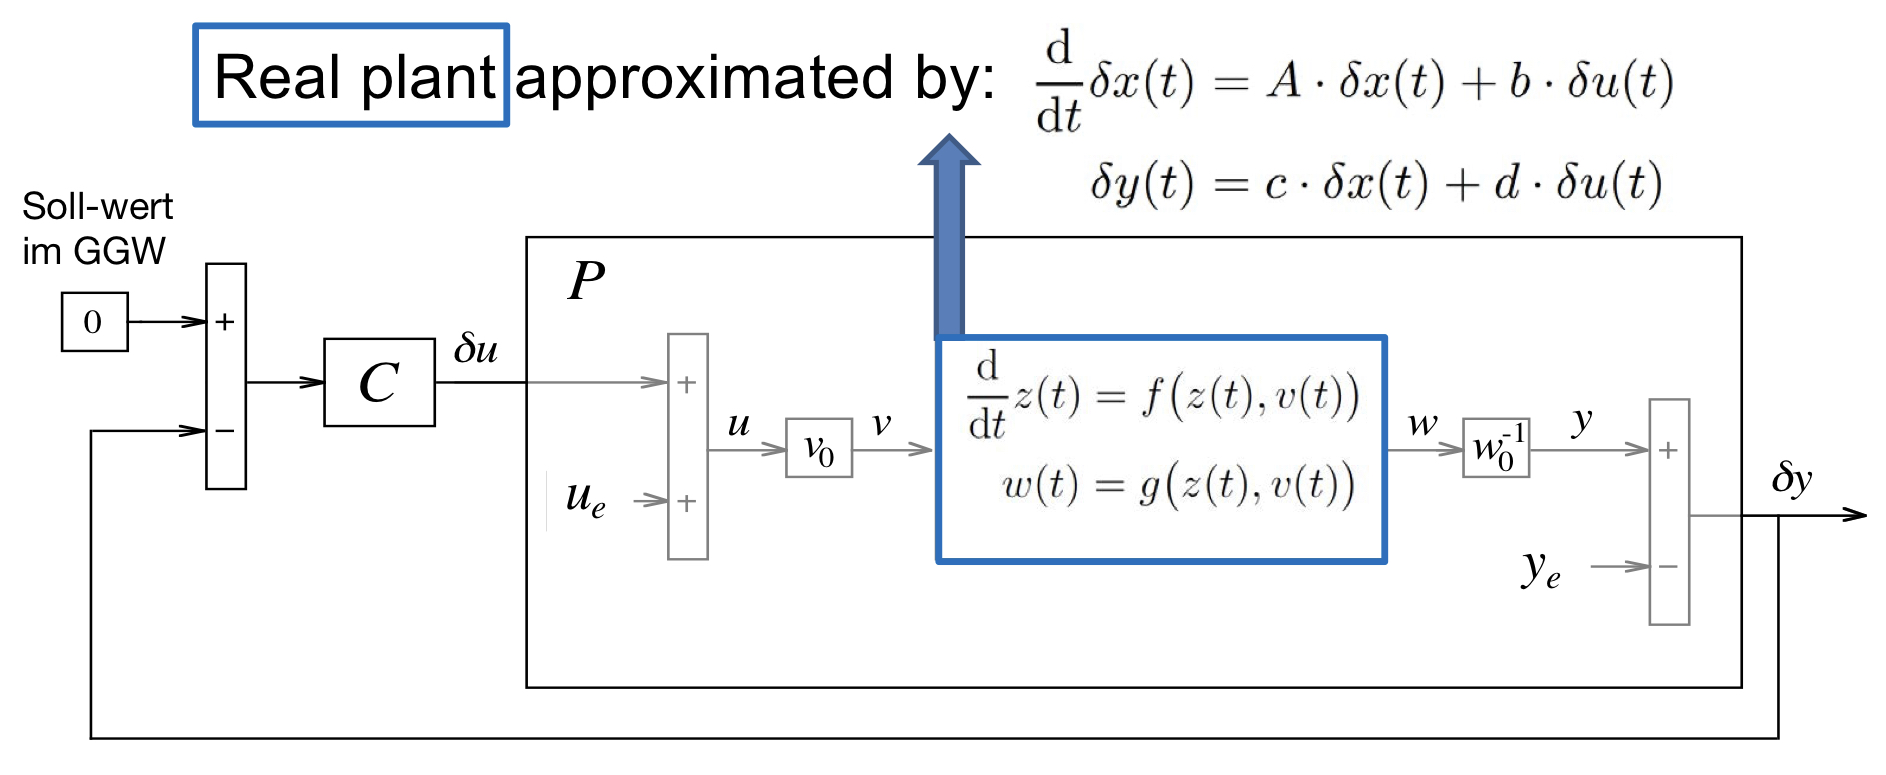
\includegraphics[width=0.8\linewidth]{02/entlinearisierung.jpg}
        \end{center}
    
    \subsubsection{Bsp}
        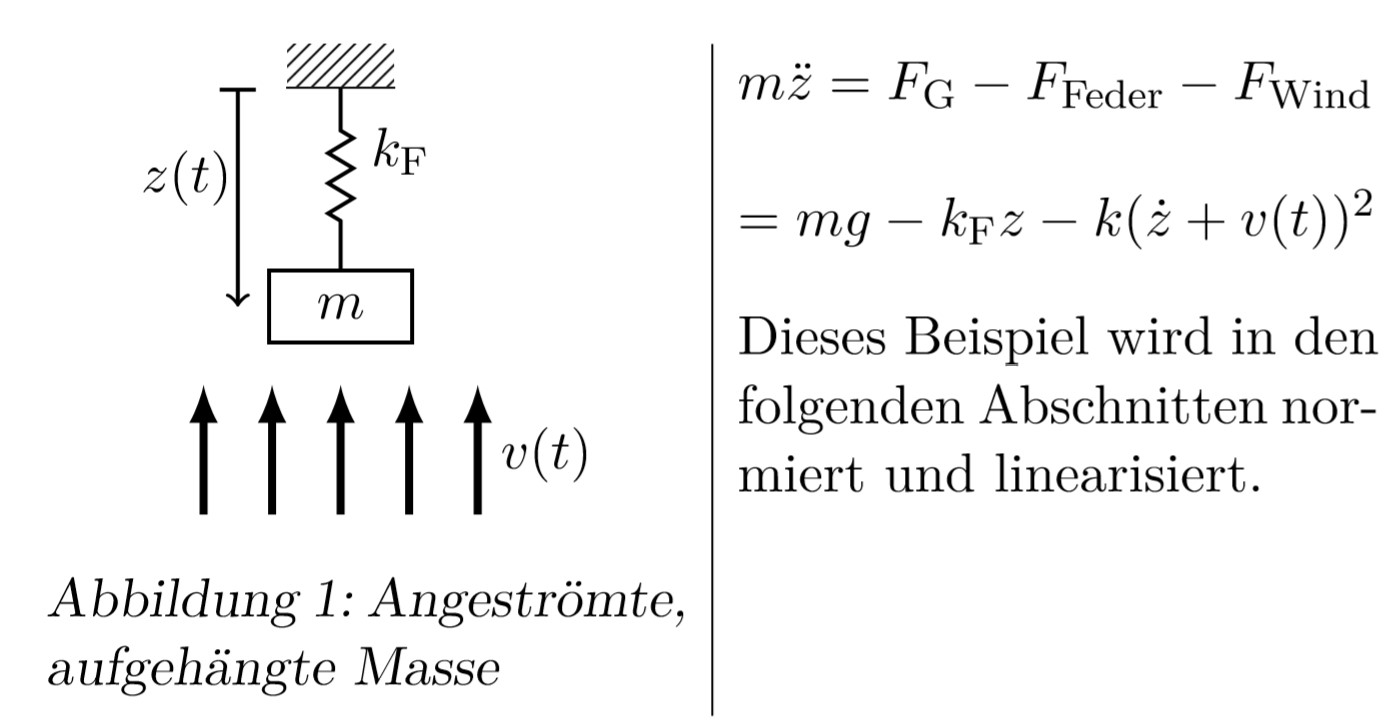
\includegraphics[width=\linewidth,     height=45mm]{images/01/01_bsp.jpg}
        \vspace{-6mm}
        
        \textbf{\underline{Zustandsgleichung:}}
            \[\frac{1}{m}(mg-k_\textrm{F}z-k(\dot{z}+v(t))^2 = \ddot{z}\]
	        \[\vec{z} = \begin{bmatrix} z\\ \dot{z} \end{bmatrix} = \begin{bmatrix} z_1\\ z_2 \end{bmatrix}\]
	        
	        \[\dot{z} = \begin{bmatrix} \dot{z}_1 \\ \dot{z}_2 \end{bmatrix} = \begin{bmatrix} z_2 \\ \frac{1}{m}(mg-k_\textrm{F}z_1-k(z_2+v(t))^2 \end{bmatrix}\]
        \textbf{\underline{Normierung:}}
            
            Es liegt im Interesse des Betrachters, dass die normierte Position $x_1$ der Masse $m$ im Gleichgewichtszustand $p_e$ (bei Wind $v_e$), $x_{1,e} = 1$ entspreche. Ausserdem weiss der Betrachter, dass gilt: $0 < v(t) < v_{max}$. Dies ist hilfreich, um die Eingangsgrösse in die Region $0 < u(t) < 1$ zu normieren. Die maximale Geschwindigkeit $\dot{z}_{max}$ sei $h$:
            
            \[ T = \begin{bmatrix} p_e & 0 \\ 0 & h \end{bmatrix}, \hspace{5mm} v(t) = v_{max} \cdot u(t)\]
            \[\dot{x} = \begin{bmatrix} \frac{h}{p_e}\cdot x_2 \\ \frac{1}{h \cdot m}(mg-k_\textrm{F} \cdot p_e \cdot x_1 - k(h\cdot x_2+v_{max} \cdot u(t))^2)\end{bmatrix} \]
            
        \textbf{\underline{Linearisierung:}}
            
            \[\dot{x}_e = \begin{bmatrix}\frac{h}{p_e}\cdot x_{2,e} \\ \frac{1}{h \cdot m}(mg-k_\textrm{F} \cdot p_e \cdot x_{1,e} - k(h\cdot x_{2,e}+v_{max} \cdot u_e)^2)\end{bmatrix} \]	
            \[= \begin{bmatrix} 0 \\ 0\end{bmatrix} \Rightarrow x_{2,e} = 0, \hspace{3mm} u_e = \frac{1}{v_{max}}\sqrt{\frac{1}{k}(mg-k_\textrm{F}p_e\cdot x_{1,e}}), \]
            
            mit $x_{1,e}=1$.
            	
            Um das System um den Gleichgewichtspunkt zu linearisieren, werden die Matrizen A,b,c,d berechnet:
            \[A = \begin{bmatrix} 0 & \frac{h}{p_e} \\ -\frac{1}{h \cdot m} \cdot k_\textrm{F} \cdot p_e & -\frac{1}{m}\cdot 2k \cdot(h\cdot x_{2,e} + v_{max} \cdot u_e) \end{bmatrix},\]
            
            \[ b = \begin{bmatrix} 0 \\ -\frac{1}{h\cdot m} \cdot 2k \cdot v_{max} \cdot (h\cdot x_{2,e} + v_{max} \cdot u_e) \end{bmatrix}\]
             
             \[ c = \begin{bmatrix} 1 & 0 \end{bmatrix}; \quad d = 0\]

    \subsubsection{Bsp}
            \[\begin{cases}
            \dot{x}_1=x_2\\
            \dot{x}_2=-2x_1-3x_2+10u\\
            y= x_1
            \end{cases}
            \]
        \[\Downarrow{Simulink-Modell}\]
        \begin{center}
            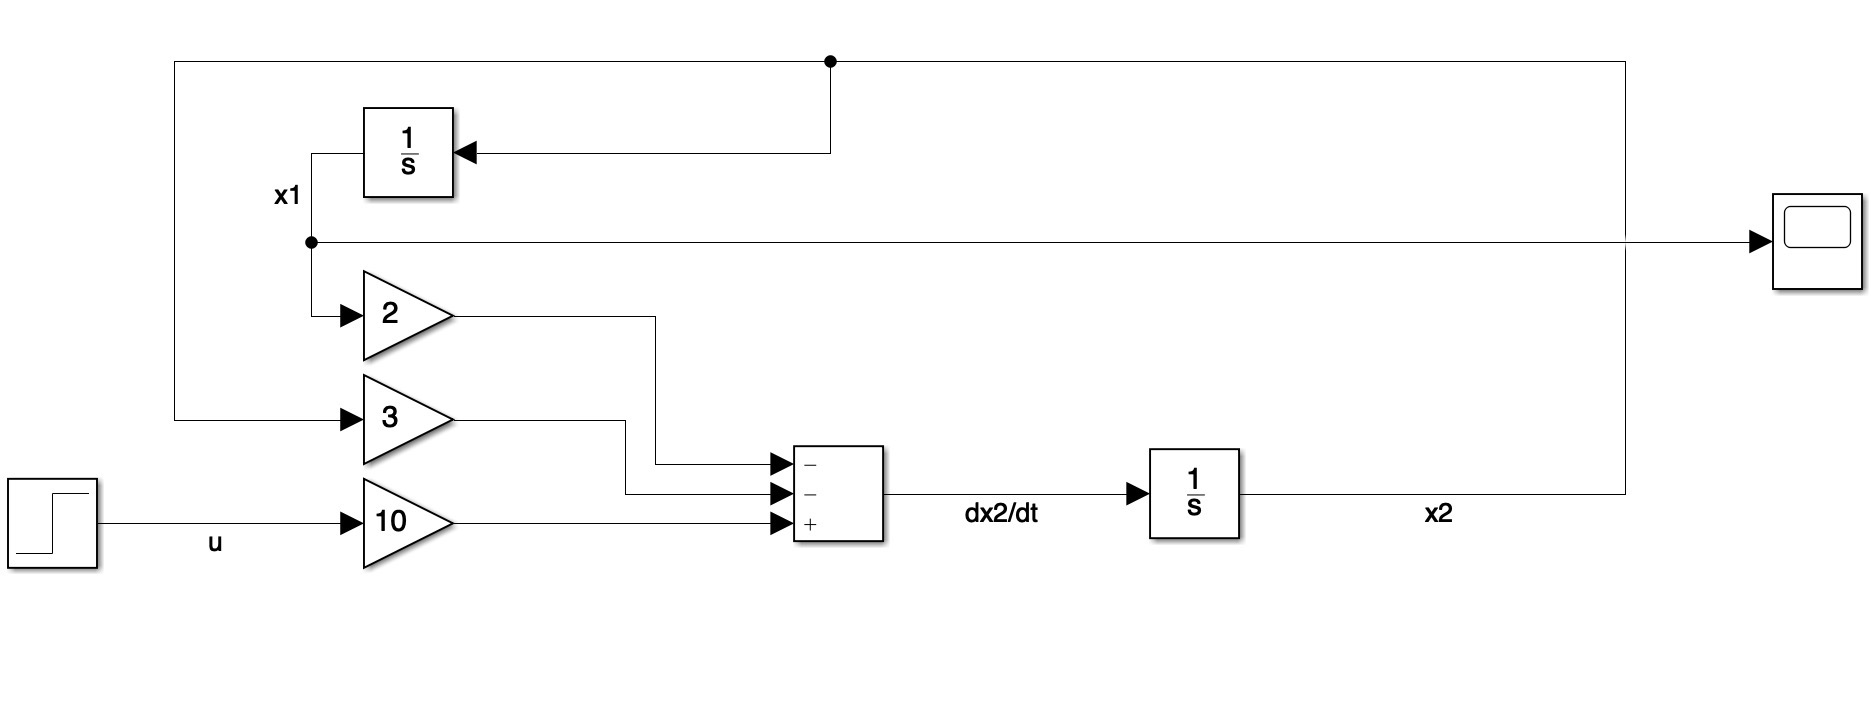
\includegraphics[width=0.8\linewidth]{images/02/simulink.jpeg}
        \end{center}
        \[\Downarrow{State\textrm{-}Space\textrm{ }Matrizen}\]
        \[A= \begin{bmatrix}
            0 & 1 \\ -2 & -3
        \end{bmatrix};\quad b=
        \begin{bmatrix}
        0\\10
        \end{bmatrix}
        \]
        \[c=\begin{bmatrix}
        1 & 0
        \end{bmatrix};\quad d=0\]
        
        